\section{What the patents are worth}\label{sec:values}

Survival is a coarse measure: it ignores how much fees differ between offices and over a patent's life. Renewal
models turn each patent's fee path and lapse decision into money. Fees come from official schedules for each of the
ten offices by year of life and period, deflated to 2024 prices with each country's consumer price index and
converted at 2024 purchasing-power parities \citep{WDI}.

\paragraph{Two models.} In the deterministic model \citep{SchankermanPakes1986}, a patent earns $r_0 d^t$ in year $t$
after grant, with $\ln r_0 \sim N(\alpha_g + \gamma \ln(1+c), \sigma)$ for owner group $g$ (domestic or foreign
$\times$ firm size or university). With returns falling and fees rising, the owner renews while returns over the
period a fee covers exceed the fee. In this model the rate of decline $1-d$ is not identified, so I also estimate the
learning model of \citet{Pakes1986}, in which log returns follow a random walk whose shocks shrink as owners learn,
and owners may keep a patent worth less than its fee for the option of later renewals. Where fees rise steeply every
year the decay rate is identified: 0.851 in Germany and 0.840 in the United Kingdom, close to the 0.85 commonly
assumed. I fix $d = 0.85$ everywhere. Appendix~\ref{app:models} gives the details.

\paragraph{The home premium is no smaller in most emerging markets.} Domestic owners value their patents more than
foreign owners in the same office, as they should: the home market is where they sell. The question is whether that
home premium is smaller in emerging markets. Figure~\ref{fig:values} shows that for China, Korea and the Czech
Republic it is not. At equal citations, the median small domestic firm's patent is worth 1.9 times the median small
foreign firm's in China, 2.0 times in Korea and 1.8 times in the Czech Republic, against 0.9--3.9 in the
advanced-economy offices. Small Taiwanese firms sit at the bottom of that range, at 0.9, while larger Taiwanese firms
and universities are well above it. Chinese universities are the exception, at 0.4. The Russian estimates are not
identified: domestic owners paid very low fees, about \$50--150 a year in PPP terms, but let many patents lapse,
while foreign owners paid four and a half times the resident fee until 2012 and kept theirs. Read literally, the model
values foreign-owned Russian patents at eight times domestic ones, with an implausibly wide spread of initial values in
the learning model. Russian patents that lapse despite near-zero fees point to low value or to lapses unrelated to the
fee, and the model cannot separate the two.

\begin{figure}[t]
\centering
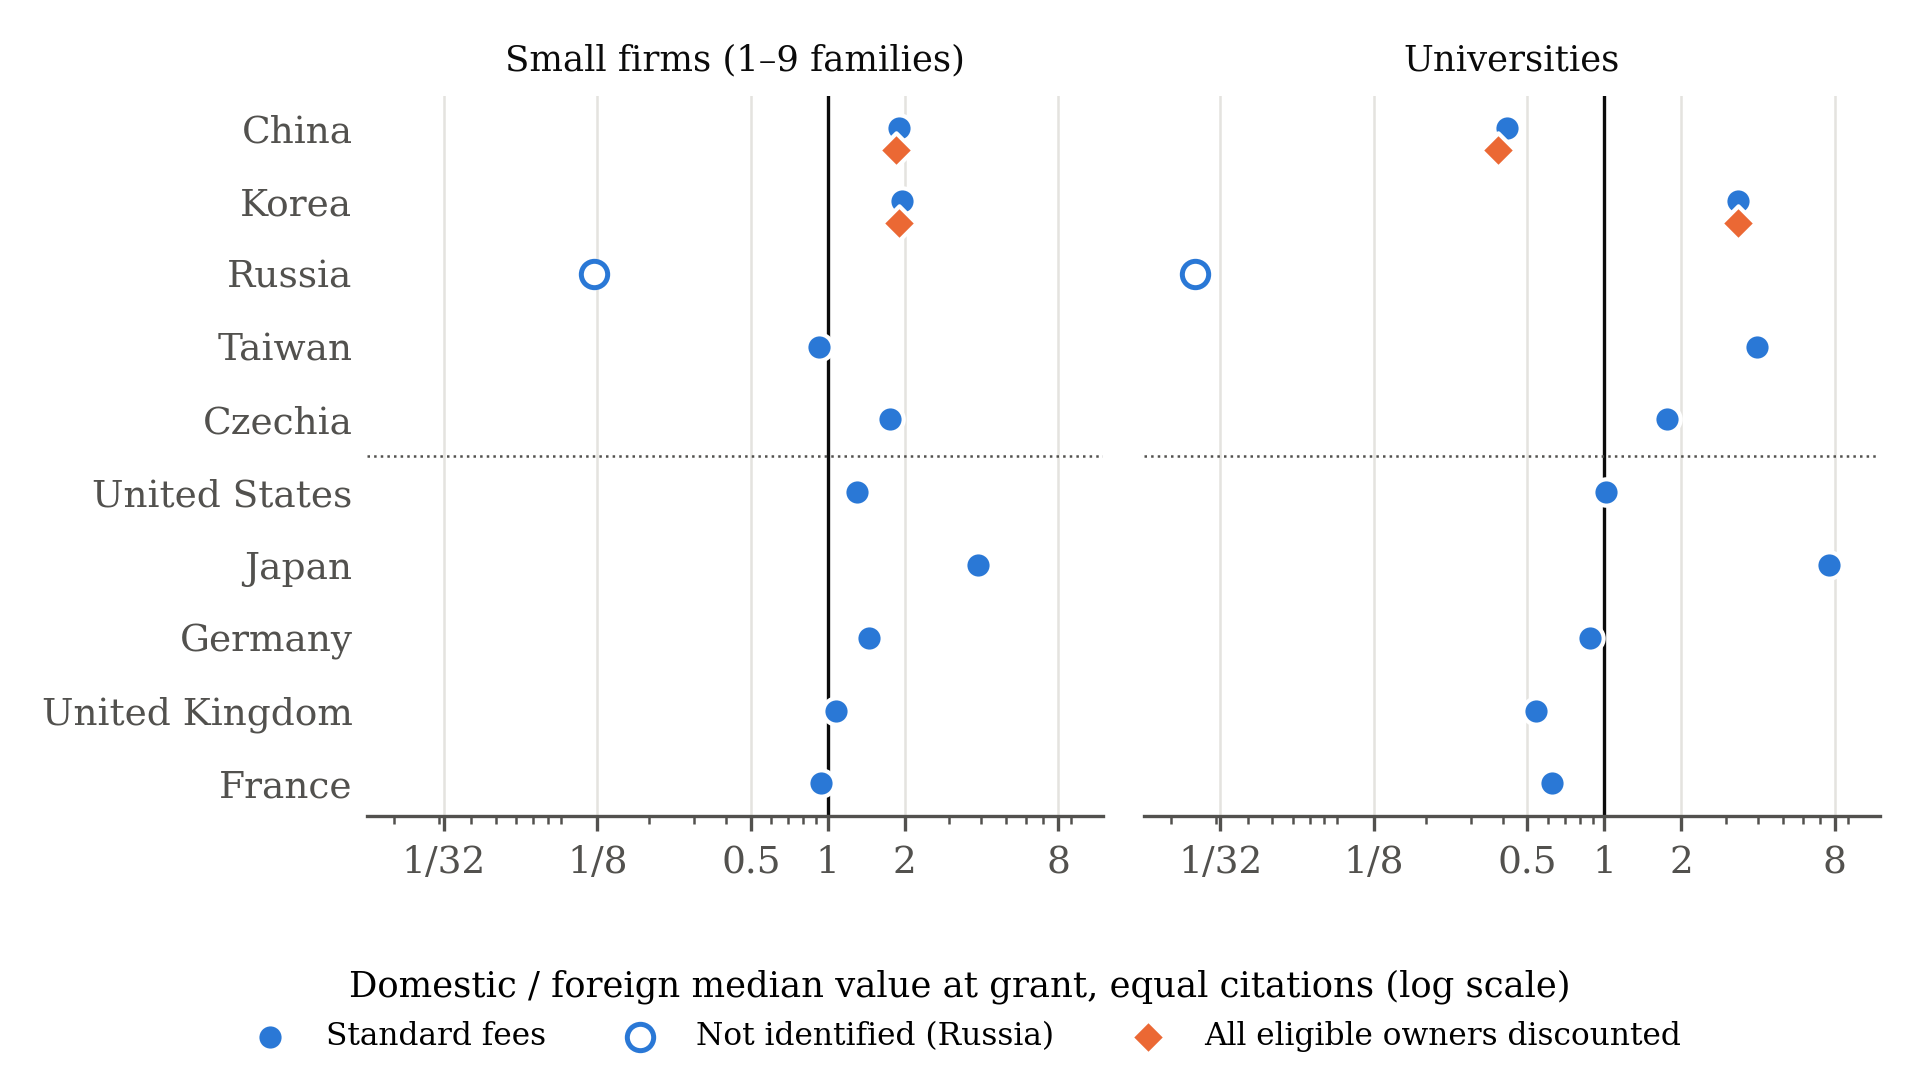
\includegraphics[width=0.9\textwidth]{figures/fig4_value_ratios.png}
\caption{Value of domestic relative to foreign owners' patents in the same office}\label{fig:values}
\figurenotes{Ratio of domestic to foreign owners' median patent value at grant, with citations at the office median,
from the deterministic renewal model ($d=0.85$, discount factor 0.9, fees in 2024 PPP dollars). Filled circles:
standard fees. Diamonds: every eligible domestic owner (firms with 1--99 families and universities) pays the
discounted fee in China and Korea, a lower bound for domestic values. Open circles: Russia, where the model is not
identified (see text). Log scale.}
\end{figure}

\paragraph{Fee discounts do not explain it.} China and Korea cut renewal fees for domestic small firms and
universities, and the models above assume standard fees. Lower fees mean the same renewal behaviour implies lower
values, so I re-estimate both models assuming that every eligible owner took the discount: in China, 30\% of the fee
in the first three fee-years after grant until 2016 and 15\% for up to ten years from 2018; in Korea, 70\% of the fee
in years 4--6 from 2014 and half from 2018. Values fall by a few percent (Figure~\ref{fig:values}): the ratio for
small firms is 1.85 in China and 1.91 in Korea in the deterministic model, and 1.61 and 1.51 in the learning model.
The discounts apply when fees are low, about \$250--350 a year in China, against values in the tens of thousands.

\paragraph{Patent-level values.} Group means could hide the patents that matter. I therefore value each patent from
its own renewal history: the learning model is re-estimated with a single prior for all owners, in which only
citations enter, and each patent's value is the posterior median over simulated return paths, weighting each path by
the probability of the patent's observed lapse or survival. Owner type plays no role in a patent's value. Regressing
log value on domestic owner by size, with fee-path $\times$ citation-band and office $\times$ field effects,
Table~\ref{tab:patentvalues} shows that small domestic firms' patents are worth about 20\% more than small foreign
firms' in China and 30\% more in Korea, as in the United States and Germany, and the same in the Czech Republic and
France. In Taiwan they are worth 18\% less. Chinese universities' patents are worth 58\% less than foreign
universities' ($1-e^{-0.87}$).

\begin{table}[t]
\centering
\begin{threeparttable}
\caption{Patent-level values, domestic minus foreign owners (log points)}\label{tab:patentvalues}
\small
% Source: em-patent-value output/patent_value_gaps.csv, patent_value_gaps_RU_TW_CZ_FR.csv (21_patent_values.py)
\begin{tabular}{lcc@{\hspace{2.5em}}lcc}
\toprule
Office & Small firms & Universities & Office & Small firms & Universities \\
\midrule
China          & 0.20 (0.03)    & $-0.87$ (0.07) & United States  & 0.22 (0.02)    & 0.13 (0.20) \\
Korea          & 0.26 (0.06)    & 0.44 (0.19)    & Japan          & 1.11 (0.07)    & 1.94 (0.55) \\
Russia\tnote{a} & $-0.45$ (0.64) & --            & Germany        & 0.21 (0.06)    & $-0.19$ (0.33) \\
Taiwan         & $-0.20$ (0.09) & 1.77 (0.32)    & United Kingdom & $-0.05$ (0.06) & $-0.59$ (0.15) \\
Czech Republic & 0.07 (0.21)    & $-0.20$ (0.57) & France         & 0.00 (0.08)    & $-0.48$ (0.27) \\
\bottomrule
\end{tabular}
\begin{tablenotes}\footnotesize
\item \emph{Notes:} Posterior median value at grant of each patent from the learning model with a common prior
($d=0.85$; 2024 PPP dollars), regressed on domestic owner $\times$ owner group with fee-path $\times$ citation-band and
office $\times$ field effects; standard errors clustered by owner. 1.37 million patents. Japanese university estimates
are unstable across specifications.
\item[a] Not identified (see text); no foreign university patents in the Russian estimation sample.
\end{tablenotes}
\end{threeparttable}
\end{table}

\paragraph{Levels are rough; ratios are not.} A typical small domestic firm's patent is worth roughly
\$5{,}000--60{,}000 at grant in the deterministic model and several times more in the learning model, in which early
lapses reflect learning rather than low initial value. Values in different offices also cover protection in
different markets. The ratios, on which the argument rests, are stable across models, decay rates and fee
assumptions, except in Russia. Because a patent's value on a given fee path rises with how long it is kept, the
patent-level values restate the survival results in money rather than adding an independent test.
